% Ctrl + alt + b to build & preview (Linux)
\documentclass[11pt,a4paper]{article}

\usepackage[margin=1in, paperwidth=8.3in, paperheight=11.7in]{geometry}
\usepackage{amsfonts}
\usepackage{amsmath}
\usepackage{enumerate}
\usepackage{enumitem}
\usepackage{fancyhdr}
\usepackage{graphicx}
\usepackage{mathtools}
\usepackage{setspace}

\begin{document}

\pagestyle{fancy}
\setlength\parindent{0pt}
\allowdisplaybreaks

\renewcommand{\headrulewidth}{0pt}
\newcommand{\vect}[1]{\boldsymbol{#1}}
\newcommand{\dotprod}[0]{\boldsymbol{\cdot}}
\newcommand{\real}[0]{\mathbb{R}}
\newcommand{\field}[0]{\mathbb{F}}
\newcommand{\naturals}[0]{\mathbb{N}}
\newcommand{\complex}[0]{\mathbb{C}}
\newcommand{\innerproduct}[2]{\langle #1, #2 \rangle}
\newcommand{\subtitle}[1]{\underline{\textit{#1}}\\}
\newcommand{\cosec}[0]{\mathrm{cosec}}

% Cover page title
\title{Calculus 1 - Application Notes}
\author{Dom Hutchinson}
\date{\today}
\maketitle

% Header
\fancyhead[L]{Dom Hutchinson}
\fancyhead[C]{Calculus 1 - Application Notes}
\fancyhead[R]{\today}

\textbf{How to Derive the Derivative of a Function.}\\

\subtitle{Theory}
The derivative of a function, $f(x)$, is defined to be
$$f'(x) := \lim_{h \to 0}\frac{f(x+h)-f(x)}{h}$$
The derivative gives you a function for the gradient at a given point.\\

\subtitle{Process}
Expanding the numerator will usually cause the $h$ in the denominator to disappear. Any terms which still have an $h$ in them can be discounted as they will tend to $0$.\\
\textit{L'H\^opital's Rule} is often useful
$$\lim_{x\to a} \frac{f(x)}{g(x)} = \lim_{x \to a}\frac{f'(x)}{g'(x)}$$

\subtitle{Example}
Find the derivative of $f(x) = (1-x^2)^2$
\[\begin{array}{rcl}
f'(x) &=& \lim_{h\to 0} \displaystyle{\frac{(1-(x+h))^2 - (1-x^2)^2}{h}}\\
&=& \lim_{h \to 0} \displaystyle{\frac{1 - 2(x+h)^2 + (x+h)^4 -(1-2x^2 + x^4)}{h}}\\
&=& \lim_{h \to 0} \displaystyle{\frac{-2\left[ x^2 + 2xh +h^2\right] +\left[x^4 + 4x^3 + 6x^2h + 4xh^3 +h^4\right] + x^2 - x^4}{h}}\\
&=& \lim_{h \to 0} \displaystyle{\frac{-4xh -2h^2 +4x^3h + 6x^2h^2 +4xh^3 + h^4}{h}}\\
&=& \lim_{h \to 0} -4x-2h+4x^3+6x^2h+4xh^2+h^3\\
&=&-4x+4x^3\\
f'(x) &=& \underline{4x\left(x^2 - 1\right)}
\end{array}\]

\textbf{Techniques for Finding the Derivative.}\\

\subtitle{Sum Rule}
\begin{center}$(f + g)' = f' + g'$\end{center}

\subtitle{Example}
Find the derivative of $(2x + x^3)$.
\[\begin{array}{rcl}
(2x + x^3)' &=& (2x)' + (x^3)'\\
&=& \underline{2 + 3x^2}
\end{array}\]

\newpage
\subtitle{Product Rule}
\begin{center}$(fg)' = f'g + fg'$\end{center}

\subtitle{Example}
Find the derivative of $2xsin(x)$.
\[\begin{array}{rcl}
(2x\sin(x))' &=& (2x)'\sin(x) + 2x(\sin(x))'\\
&=& \underline{2\sin(x) + 2x\cos(x)}
\end{array}\]

\subtitle{Quotient Rule}
\begin{center}$\displaystyle{\left(\frac{f}{g}\right)' = \frac{f'g - fg'}{g^2}}$\end{center}

\subtitle{Example}
Find the derivative of $\displaystyle{\frac{2x}{\sin(x)}}$.
\[\begin{array}{rcl}
\displaystyle{\left(\frac{2x}{\sin(x)}\right)'} &=&\displaystyle{\frac{(2x)'\sin(x) - 2x(\sin(x))'}{\sin^2(x)} }\\
&=& \displaystyle{\frac{2\sin(x) - 2x\cos(x)}{\sin^2(x)}}\\
&=& \displaystyle{2\left[\frac{1}{\sin(x)} - \frac{x}{\tan(x)\sin(x)}\right]}\\
&=& \underline{\displaystyle{2\cosec(x) \left[1 - x\cot(x) \right]}}
\end{array}\]

\subtitle{Chain Rule}
\begin{center}$f(g(x))' = f'(g(x))g'(x)$\end{center}

\subtitle{Example}
Find the derivative of $\sin(2x)$.
\[\begin{array}{rcl}
f(x) = \sin(x) &\implies& f'(x) = \cos(x)\\
g(x) = 2x &\implies& g'(x) = 2\\
\implies sin(2x)' &=& \underline{2\cos(2x)}
\end{array}\]\\

\textbf{How to Find the Derivative of an Equation Where Elements Cannot be Easily Seperated.}\\

\subtitle{Theory}
Remember that $\frac{d}{dx}(x) = 1\ \&\ \frac{d}{dx} y = \frac{dy}{dx}  = y'$.\\
By the chain rule $\left(\frac{1}{dx}\right)(dy) = \frac{dy}{dx}\ \&\ \frac{dx}{dy} = \frac{1}{dy/dx}$.\\

\subtitle{Process}
Differentiate both sides with respect to the same variable.\\
 to form an equation in termins of the given gradient$\left(\frac{dx}{dy}, \frac{dy}{dx},\ \mathrm{etc.}\right)$

\subtitle{Example}
Find $\frac{dy}{dx}$ of $x^3 + y^3 = xy$.
\[\begin{array}{rrcl}
& \frac{d}{dx}\left(x^3 + y^3\right) &=& \frac{d}{dx}\left(xy\right)\\
\implies& 3x^2 + 3y^2\frac{dy}{dx} &=& y + x\frac{dy}{dx}\\
\implies& \frac{dy}{dx}\left(x - 3y^2\right) &=& 3x^2 - y\\
\implies& \displaystyle{\frac{dy}{dx}} &=& \displaystyle{\underline{\frac{3x^2-y}{x-3y^2}}}
\end{array}\]

\textbf{How to Find the Tangent to a Parametric Curve}\\

\subtitle{Process}
Use the following formula gives the tangent when $t = t_0$ as a cartesian equation.
$$\displaystyle{\frac{dy/dt}{dx/dt}}(t_0) = \displaystyle{\frac{y - y(t_0)}{x-x(t_0)}}$$

\subtitle{Example}
Find the tangent of $x = t^4 + 1\ \&\ y=t^2+t$ when $t = 1$.
\[\begin{array}{rrclcl}
&\frac{dy}{dt} &=& 2t + 1\\
&\frac{dx}{dt} &=& 4t^3\\
\implies&\frac{dy/dt}{dx/dt}(1) &=& \frac{2(1) + 1}{4(1)} &=& \frac{3}{4}\\
\mathrm{Set}&\frac{3}{4} &=& \frac{y-y(1)}{x-x(1)}\\
&&=& \frac{y - (1^2 + 1)}{x - (1^4 + 1)}\\
&&=& \frac{y-2}{x-2}\\
\implies& \frac{3x}{4} - \frac{6}{4} &=& y - 2\\
\implies& y &=& \underline{\frac{3x}{4} - \frac{1}{2}}
\end{array}\]

\textbf{How to Find the Arc-Length of a Parametric Curve}\\

\subtitle{Process}
The legth of $(x(t), y(t))$ for $a \leq t \leq b$ is found with
$$s = \int_a^b \sqrt{\left(\frac{dx}{dt}(t)\right)^2 + \left(\frac{dy}{dt}(t)\right)^2}dt$$

\subtitle{Example}
Find the arc-legth of $(3\cos(t), 3\sin(t))$ for $t \in \left[0, \frac{\pi}{2}\right]$.
\[\begin{array}{rcl}
s &=& \int_0^{\frac{\pi}{2}} \sqrt{\left(-3\sin(t)\right)^2 + \left(3\cos(t)\right)^2}dt\\
&=& \int_0^{\frac{\pi}{2}} \sqrt{9\left[\sin^2(t) + \cos^2(t)\right]}dt\\
&=& \int_0^{\frac{\pi}{2}} 3 dt\\
&=& 3t\big|_0^\frac{\pi}{2}\\
&=& \underline{\frac{3\pi}{2}}
\end{array}\]

\textbf{How to Find the Curvature of A Curve}\\

\subtitle{Theory}
\textit{Curvature} measures how fast the gradient of a curve is changing at a given point.\\

\subtitle{Process}
For a cartesian curve \textit{curvature} is given by
$$K(x) = \displaystyle{\frac{|y''(x)|}{\left[1 + \left(y'(x)\right)^2\right]^{3/2}}}$$
For a parametric curve it is given by
$$K(t_0) = \displaystyle{\frac{y''(t_0)x'(t_0) - y'(t_0)x''(t_0)}{\left[\left(x'(t_0)\right)^2 + \left(y'(t_0)\right)^2\right]^{3/2}}}$$

\textbf{How to Solve a First-Order Differential Equation}\\

\subtitle{Theory}
A first-order differential equation takes the form
$$q(x) = p(x) + \frac{dy}{dx}$$
An integrating factor for an equation of this form is found by
$$R := e^{\int p(x)dx}$$

\subtitle{Process}
Rearrange the differential equation to the form $q(x) = p(x)y + \frac{dy}{dx}$.\\
Calculate the integrating factor, $R$.\\
Then\[\begin{array}{rrcl}
&Rq(x)&=&\frac{d}{dx}(Ry)\\
\implies& y &=& \displaystyle{\frac{\int Rq(x) dx}{R}}
\end{array}\]

\subtitle{Example}
Find a $y = f(x)$ such that $xy' + y = e^x$.
\[\begin{array}{rrcl}
\implies&R&=&e^{\int\frac{1}{x}dx}\\
&&=&e^{\ln(x)}\\
&&=&x\\
\implies& e^x &=& \frac{d}{dx}(xy)\\
\implies& y &=& \displaystyle{\frac{\int e^x dx}{x}}\\
&&=& \displaystyle{\underline{\frac{e^x + c}{x}}}
\end{array}\]

\textbf{How to Solve a Second-Order Linear Differential Equation}\\

\subtitle{Theory}
A second-order linear differential equation takes the form
$$ay + b\frac{dy}{dx} + c\frac{d^2y}{dx^2} = d(x)$$
The \textit{complementary function}, $y_c$, is a solution to $ay + b\frac{dy}{dx} + c\frac{d^2y}{dx^2} = 0$.\\
The \textit{particular function}, $y_p$, is a solution to $ay + b\frac{dy}{dx} + c\frac{d^2y}{dx^2} = d(x)$.\\

\subtitle{Process}
Rearrange the differential equation to the form $ay + b\frac{dy}{dx} + c\frac{d^2y}{dx^2} = d(x)$.\\

\textit{Complementary function}.\\
Set $a\lambda^2 + b\lambda + c = 0$\\
Solve this to find $\lambda_1\ \&\ \lambda_2$.\\
The form of $\lambda_1\ \&\ \lambda_2$ defines the form of the complementary function.\\
If\\
\-\hspace{4ex}$\lambda_1 = \lambda_2 \in \real \implies y_c = \mu_1 e^{\lambda_1 x} + \mu_2xe^{\lambda_1 x}$;\\
\-\hspace{4ex}$\lambda_1, \lambda_2 \in \real \implies y_c = \mu_1 e^{\lambda_1 x} + \mu_2 e^{\lambda_2 x}$;\\
\-\hspace{4ex}$\lambda_1, \lambda_2 \in i\real \implies y_c = \mu_1 \cos\left(\frac{\lambda_1}{i}\right) + \mu_2 \cos\left(\frac{\lambda_2}{i}\right)$; or\\
\-\hspace{4ex}$\lambda_1, \lambda_2 \in \complex\ \&\ Re(\lambda_1) \neq 0 \implies y_c = e^{Re(\lambda_1)x}\left[\mu_1 \cos(Im(\lambda_1) + \mu_2 \cos(Im(\lambda_1)\right]$.
\underline{N.B.} - These are all just $\mu_i e^{\lambda_i x}$ in Euler's Form.\\

\textit{Particular function}.\\
Establishing a general particular solution.\\
This depends on the form of $d(x)$.\\
If\\
\-\hspace{4ex}$d(x) = a_nx^n + \dots + a_1x + a_0$ set $y_p = b_nx^n + \dots + b_1x+b_0$;\\
\-\hspace{4ex}$d(x) = ae^{bx}$ set $y_p = ce^{dx}$; or\\
\-\hspace{4ex}$d(x) = a\sin(bx) + c\cos(dx)$ set $y_p = f\sin(gx) + h\cos(jx)$.
Differentiate the general $y_p$ twice to get $y_p'$ and $y_p''$.\\
Substitute these into the original equation, in place of the $y$s.\\
Solve this to find values for the constants in $y_p$.\\
Finally, $y  =y_c + y_p$.\\
Initial conditions are required to find values for the constants in $y_c$.\\

\subtitle{Example}
Find $y = f(x)$ such that $10y'' - y = e^x$.\\
\[\begin{array}{rrcl}
\mathrm{Set}& 10\lambda^2 + 0\lambda - 1 &=& 0\\
\implies& 10\lambda^2 &=& 1\\
\implies& \lambda &=& \pm \frac{1}{\sqrt{10}}\\
&\lambda \in \real\ \mathrm{so}\ y_c &=& \mu_1 e^{\frac{x}{\sqrt{10}}} + \mu_2 e^{-\frac{x}{\sqrt{10}}}\\
\mathrm{Set}& y_p &=& ae^x\\
\implies& y_p' &=& ae^x\\
\&& y_p'' &=& ae^x\\
\implies& 10ae^x - ae^x &=& e^x\\
\implies& 9a &=& 1\\
\implies& a &=& \frac{1}{9}\\
\implies& y &=& \underline{\frac{1}{9}e^x +  \mu_1 e^{\frac{x}{\sqrt{10}}} + \mu_2 e^{-\frac{x}{\sqrt{10}}}}
\end{array}\]

\newpage\textbf{How to Solve Inhomogenous Second-Order Differential Equations using the Wronskian}\\

\subtitle{Theory}
A second-order differential equation is \textit{inhomogenous} if $y''(x) + ay'(x) + by(x) = d(x)$ with $d \neq 0$.\\
A \textit{Wronskian Matrix} is defined as
$$\Phi[y_1, \dots, y_n] := \begin{pmatrix} y_1 & y_2 & \dots & y_n \\ y_1' & y_2' & \dots & y_n' \\ \vdots & \vdots & \ddots & \vdots \\ y_1^{(n-1)} & y_2^{(n-1)} & \dots & y_n^{(n-1)} \end{pmatrix}$$
The \textit{Wronskian} is defined as
$$W[y_1, \dots, y_n] := det(\Phi[y_1, \dots,y_n]) = \begin{vmatrix} y_1 & y_2 & \dots & y_n \\ y_1' & y_2' & \dots & y_n' \\ \vdots & \vdots & \ddots & \vdots \\ y_1^{(n-1)} & y_2^{(n-1)} & \dots & y_n^{(n-1)} \end{vmatrix}$$
If $W[y_1, \dots, y_n] \neq 0$ then $y_1, \dots, y_n$ are linearly independent.\\

\subtitle{Process}
Rearrange the differential equation to the form $y + a\frac{dy}{dx} + b\frac{d^2y}{dx^2} = c(x)$.\\
Find the complementary function, $y_c$, of this equation, as shown earlier.\\
$y_c$ will have the form $y_c = \lambda_1z_1(x) + \lambda_2z_2(x)$ where $z_1(x)$ \& $z_2(x)$ are linearly independent.\\
Define the particular solution to be $y_p = \mu_1(x)z_1(x) + \mu_2(x)z_2(x)$.\\
Then $\mu_1'(x)=\frac{\begin{vmatrix} 0 & z_2(x) \\ c(x) & z_2(x)'\end{vmatrix}}{W[z_1(x), z_2(x)]} = \frac{-x_2(x)c(x)}{W[z_1(x), z_2(x)]}$ and $\mu_2'(x)=\frac{\begin{vmatrix} z_1(x) & 0 \\ z_2(x)' & c(x)\end{vmatrix}}{W[z_1(x), z_2(x)]} = \frac{z_1(x)c(x)}{W[z_1(x), z_2(x)]}$.\\
Use integration to find $\mu_1(x)$ \& $\mu_2(x)$.\\
Finally $y = \mu_1(x)z_1(x) + \mu_2(x)z_2(x)$.\\

\newpage\subtitle{Example}
Find $y=f(x)$ such that $y''-y=x$.\\
\[\begin{array}{rrcl}
\mathrm{Set}& \lambda^2-1&=&0\\
\implies& \lambda^2 &=&1\\
\implies&\lambda_1 = 1 &\&& \lambda_2 = -1\\
\mathrm{Set}& y_c &=& \mu_1e^x + \mu_2e^{-1}\\
\\\mathrm{So}& z_1(x) = e^x &\&& z_2(x) = e^{-x}\\
&W[z_1(x), z_2(x)] &=& \begin{vmatrix} e^x & e^{-x} \\ e^x & -e^{-x} \end{vmatrix}\\
&&=& -1 - 1\\
&&=& -2\\
\implies& \mu_1'(x) &=& \displaystyle{\frac{\begin{vmatrix}0 & e^{-x} \\ x & -e^{-x} \end{vmatrix}}{-2}}\\
&&=& \displaystyle{\frac{-xe^{-x}}{-2}}\\
&&=& \displaystyle{\frac{xe^{-x}}{2}}\\
\&& \mu_2'(x) &=& \displaystyle{\frac{\begin{vmatrix}e^x & 0 \\ e^x & 0 \end{vmatrix}}{-2}}\\
&&=& \frac{-xe^x}{2}\\
\implies& \mu_1 &=& -\frac{1}{2}(1+x)e^{-x}\\
\&& \mu_2 &=& \frac{1}{2}(1-x)e^x\\
\implies& y &=& (-\frac{1}{2}(1+x)e^{-x})e^x + (\frac{1}{2}(1-x)e^x)e^{-x}\\
&&=& -\frac{1}{2}(1+x) + \frac{1}{2}(1-x)\\
&y &=& \underline{-x}
\end{array}\]

\textbf{How to Solve a First-Order linear Difference Equations}\\

\subtitle{Theory}
A first-order linear difference equation takes the form
$$y_{n+1} = f + ay_n$$
where $y_n\ \&\ y_{n+1}$ are part of a sequence.\\
This is a recursive function so requires a stopping condition.\\
Geometric progressions, $\{a, ar, ar^2, \dots \}$, are a first-order linear difference equation where $f = 0$.\\
The sum of the first $n$ terms of a geometric progression is $\frac{a(1-r^n)}{1-r}$.\\

\subtitle{Process}
Rearrange the equation to the form $y_{n+1} = ay_n + b$.\\
\[\begin{array}{rrcl}
\implies& y_{n+1} &=& a[ay_{n-1} + b] + b\\
&&=& b[1 + a] + a^2y_{n-1}\\
\implies& y_{n+1} &=& b[1 + a + \dots + a^{n-1}] + a^ny_1
\end{array}\]
Since $1 + a + \dots + a^{n-1}$ is a geometric sequence then\\
\-\hspace{4ex}$y_{n+1} = b\left[\frac{1-a^{n-1}}{1-a}\right] + a^ny_1$\\
This is now solved.\\

\subtitle{Example}
Find $y_n = f(n)$ such that $3y_{n+1} + y_n = 15$.
\[\begin{array}{rrcl}
\implies& y_{n+1} &=& 5 - \frac{1}{3}y_n\\
&&=& 5\left[1 - \frac{1}{3}\right] + \left[\frac{-1}{3}\right]^2.y_{n-1}\\
&&=& 5\left[1 - \frac{1}{3}\right] + \dots + \left(\frac{-1}{3}\right)^n] + \left[\frac{-1}{3}\right]^n.y_0\\
&&=& 5\left[\frac{1-\left(\frac{-1}{3}\right)^n}{1-\frac{-1}{3}}\right] + \left[\frac{-1}{3}\right]^n.y_0\\
&&=& \frac{15}{4}\left[1 - \left(\frac{-1}{3}\right)^n\right] + \left[\frac{-1}{3}\right]^n.y_0\\
&&=& \underline{\left(\frac{-1}{3}\right)^n\left[y_0 - \frac{15}{4}\right] + \frac{15}{4}}
\end{array}\]

\textbf{How to Solve Second-Order Linear Difference Equations}\\

\subtitle{Theory}
A second-order linear difference equation takes the form
$$ay_{n+2} + by_{n+1} + cy_n = d(n)$$
The solution for $y_n$ has two parts, a complementary \& particular solution. $y_n = y_n^c + y_n^p$.\\
The complementary equation deals with the homogenous case \& the particular equation with the inhomogenous case.\\

\subtitle{Process}
Rearrange the difference equation to form $ay_{n+2} + by_{n+1} + cy_n = d(n)$.\\
Set $a\lambda^2 + b\lambda + c = 0$.''
Solve to find $\lambda_1$ \& $\lambda_2$.
Let $y_n^c$ be the complementary function. Set it with these conditions.\\
If\\
\-\hspace{2em} $\lambda_1 = \lambda_2 \in \real \quad \quad \quad \quad \quad \quad \quad \implies y_n^c = \mu_1\lambda_1^n + n\mu_2\lambda_2^n$;\\
\-\hspace{2em} $\lambda_1, \lambda_2 \in \real\quad \quad \quad \quad \quad \quad \quad \quad \implies y_n^c = \mu_1\lambda^n + \mu_2\lambda_2^n$; or,\\
\-\hspace{2em} $\lambda_1, \lambda_2 \in \complex\ st\ \lambda_1, \lambda_2 = Re^{\pm i\theta} \implies y_n^c = R^n.[\mu_1 cos(n\theta)+\mu_2 sin(n\theta)]$.\\
Let $y_n^p$ be the particular function. Set it with these conditions.\\
If\\
\-\hspace{2em} $d(n) = a \in \real\ \forall\ n \implies y_n^p = A$;\\
\-\hspace{2em} $d(n) = an \implies y_n^p = An + B$;\\
\-\hspace{2em} $d(n) = an^2 \implies y_n^p = An^2 + Bn + C$;\\
\-\hspace{2em} $d(n) = a\sin(bn) + c\cos(bn) \implies y_n^p = A\sin(bn) + B\cos(bt)$; or,\\
\-\hspace{2em} $d(n) = cn^t\quad \implies y_n^p = An^t$.\\
Expand this to find $y_{n+1}$ \& $y_{n+2}$.\\
Substitue these into the original equation to find values for the constants, by comparing coefficients.\\
Finally, $y_n = y_n^c + y_n^p$.\\

\newpage\subtitle{Example}
Find $y_n = f(n)$ such that $y_{n+2} -4y_{n+1} + 4y_n = n$\\
\[\begin{array}{rrcl}
\mathrm{Set}& \lambda^2 - 4\lambda + 4 &=&0\\
\implies& (\lambda - 2)^2 &=&0\\
\implies& \lambda_1 = 2 = \lambda_2\\
\mathrm{Set}& y_n^c &=& \mu_12^n + n\mu2^n\\
\\\mathrm{Let}& y_n^p &=& An + b\\
\implies&y_{n+1}^p &=& A(n+1) + b\\
\&&y_{n+2}^p &=& A(n+2) + b\\
\implies& [A(n+2)+B]\\&-4[A(n+1)+B]+4[An+B] &=& n\\
\implies& An - 2A +B&=&n\\
&[n^1] : A &=& 1\\
&[n^0] : -2A+B &=& 0\\
\implies& B &=& 2A = 2\\
\implies& y_n^p &=& n + 2\\
\implies& y_n &=& \underline{n+2+\mu_12^n + n\mu2^n}
\end{array}\]

\textbf{How to Find a Directional Derivative}\\

\subtitle{Theory}figure
A \textit{direction} is a unit length vector.\\
This takes the form $\begin{pmatrix} \cos(\theta) \\ \sin(\theta) \end{pmatrix}$ in $\real^2$ \& $\begin{pmatrix} \sin(\phi)\cos(\theta) \\ \sin(\phi)\sin(\theta) \\ \cos(\phi) \end{pmatrix}$ in $\real^3$.\\
A \textit{directional derivative} gives the rate of change of a multi-variable function in a particular direction.\\

\subtitle{Process}
\-\hspace{4ex}$D_{\vect{u}}\vect{f}(\vect{x}) = \vect{f}'(\vect{x}) \dotprod \vect{u}$ where $\vect{u}$ is a direction.\\

\textbf{How to Find a Partial Derivative}\\

\subtitle{Theory}
A \textit{partial derivative} is a directional derivative where the direction is a standard basis vector.\\
So $D_{\vect{e}_j}\vect{f}(\vect{x})$ is a partial derivative.\\
This can be denoted as $D_{\vect{e}_j}\vect{f}(\vect{x}) = \vect{f}'_j(\vect{x}) = \frac{\partial f}{\partial x_j}(\vect{x})$\\
A matrix of all the partial derivatives can be formed. If $\vect{f} : \real^n \to \real^m, n \in \naturals$ then $\vect{f}' \in M_{m, n}$.\\
\begin{center}$\vect{f}'(\vect{x}) = \begin{pmatrix} \frac{\partial f_1}{\partial x_1} & \frac{\partial f_1}{\partial x_2} & \dots & \frac{\partial f_1}{\partial x_n} \\ \frac{\partial f_2}{\partial x_1} & \frac{\partial f_2}{\partial x_2} & \dots & \frac{\partial f_2}{\partial x_n} \\ \vdots & \vdots & \ddots & \vdots \\ \frac{\partial f_m}{\partial x_1} & \frac{\partial f_m}{\partial x_2} & \dots & \frac{\partial f_m}{\partial x_n}\end{pmatrix}$ \end{center}

\subtitle{Example}
Find $\vect{f}'(\vect{x})$ of $\vect{f}'(x,y,z) = (x, 2x+y, z^2)$.\\
\begin{center} $\vect{f}'(\vect{x}) = \begin{pmatrix} 1 & 2 & 0 \\ 0 & 1 & 0 \\ 0 & 0 & 2z\end{pmatrix}$ \end{center}

\textbf{How to Convert Between Cartesian \& Polar Co-ordinates}\\

\subtitle{Theory}
\textit{Polar co-ordinates} describe a point in two-dimensional space in terms of its distance from the origin, $r$, and its angle from the positive x-axis, $\theta$.\\
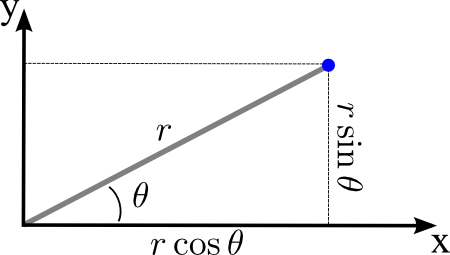
\includegraphics[scale=0.5]{polar.png}\\

\textit{\underline{Process} - Cartesian to Polar}\\
For a point $\vect{v} = \begin{pmatrix}r \\ \theta\end{pmatrix}$ in polar co-ordiantes.\\
$\vect{v} = \begin{pmatrix} r\cos(\theta) \\ r\sin(\theta) \end{pmatrix}$ in cartesian co-ordinates.\\

\textit{\underline{Process} - Polar to Cartesian}\\
For a point $\vect{v} = \begin{pmatrix} x \\ y \end{pmatrix}$ in cartesian co-ordinates.\\
\-\hspace{2em}$x=r\cos(\theta)\ \& \ y=r\sin(\theta) \implies \tan(\theta) = \frac{y}{x}\ \&\ r = \sqrt{x^2 + y^2}$\\
So $\vect{v} = \begin{pmatrix} \sqrt{x^2 + y^2} \\ \tan^{-1}\left(\frac{y}{x}\right)\end{pmatrix} = \begin{pmatrix} r \\ \theta \end{pmatrix}$ in polar co-ordinates.\\

\subtitle{Example}
\textit{Polar $\to$ Cartesian}\\
Let $\vect{v} = (60, \frac{\pi}{4})$.\\
\-\hspace{2em}$\vect{v} = \begin{pmatrix} 60\cos(\frac{\pi}{4}) \\ 60\sin(\frac{\pi}{4}) \end{pmatrix} = \begin{pmatrix} 60(\frac{1}{\sqrt{2}}) \\ 60(\frac{1}{\sqrt{2}})\end{pmatrix} = \underline{\begin{pmatrix} 30\sqrt{2} \\ 30\sqrt{2} \end{pmatrix}}$\\
\textit{Cartesian $\to$ Polar}\\
Let $\vect{v} = (-\sqrt{3}, 1)$.\\
\-\hspace{2em}$\theta = \tan^{-1}(\frac{-1}{\sqrt{3}}) = -\frac{\pi}{6}\ \&\ r = \sqrt{\sqrt{3}^2 + 1^2} = \sqrt{4} = 2$\\
$\implies\vect{v} = \underline{(2, \frac{-\pi}{6})}$.\\

\textbf{How to Convert Between Cartesian \& Sperical Co-Ordinates}\\

\subtitle{Theory}
\textit{Spherial co-ordinates} describe a point in three-dimensional space in terms of its distance from the origin, $\rho$, its angle from the positive x-axis, $\theta$, \& its angel from the positive z-axis, $\phi$.\\
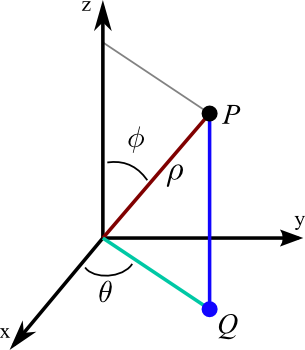
\includegraphics[scale=0.3]{spherical.png}\\

\newpage\textit{\underline{Process} - Cartesian to Spherical}\\
Let $\vect{v} = (\rho, \theta, \phi)$ in spherical co-ordinates.\\
Then $\vect{v} = \begin{pmatrix} \rho\sin(\phi)\cos(\theta) \\ \rho\sin(\phi)\sin(\theta) \\ \rho\cos(\phi) \end{pmatrix} = \begin{pmatrix} x\\y\\z \end{pmatrix}$ in cartesian co-ordiantes.\\

\textit{\underline{Process} - Spherical to Cartesian}\\
Let $\vect{v} = (x, y, z)$ in spherical co-ordinates.\\
Then $\vect{v} = \begin{pmatrix} \sqrt{x^2 + y^2 + z^2} \\ \tan^{-1}(\frac{y}{x}) \\ \cos^{-1}\left(\frac{z}{\sqrt{x^2 + y^2 + z^2}}\right) \end{pmatrix} = \begin{pmatrix} \rho\\\theta\\\phi \end{pmatrix}$ in spherical co-ordiantes.\\

\textbf{How to Find a Volume of a Region}\\

\subtitle{Theory}
Multiple integeration is used to find the volume of a region in three-dimensional space.\\
Multiple integeration involves integerating over the same region, with a multiple different variables, sequentially.\\
These can be treated as seperate integrals, processing the innermost first.\\
They are denoted by $\int_R f(\vect{x})d\vect{x}$ where $R$ is the region and $f(\vect{x})$ is a density function.\\
This can be expanded as
$$\int_{a_n}^{b_n} \left\{ \dots \int_{a_2}^{b_2} \left\{ \int_{a_1}^{b_1} f(\vect{x}) dx_1 \right\} dx_2 \dots \right\} dx_n$$
where $R = \{ \vect{x} \in \real^n : a_n \leq x_n \leq b_n, \dots, a_1 \leq x_1 \leq b_1\}$.\\

\subtitle{Process}
When wanting to find the volume of $R \subset \real^3$ set $f\vect{x} = 1$ and perform a triple integration.\\

\subtitle{Example}
Find the volume of $R = \{(x, y, z) \in \real^3 : 0 \leq x \leq 1-y-z, 0 \leq y \leq 1-z, 0 \leq z \leq 1\}$.
\[\begin{array}{rcl}
\int_D1\ dxdydz &=& \displaystyle{\int_{0}^{1} \left\{ \int_{0}^{1-z} \left\{ \int_{0}^{1-y-z} 1\ dx \right\} dy \right\} dz}\\
&=& \displaystyle{\int_{0}^{1} \left\{ \int_{0}^{1-z} 1-y-z\ dy \right\} dz}\\
&=& \displaystyle{\int_{0}^{1} y - \frac{y^2}{2} -yz \big|_0^{1-z}\ dz}\\
&=& \displaystyle{\int_0^1 1 - z - \frac{(1-z)^2}{2} -z + z^2 dz}\\
&=& \displaystyle{\int_0^1 (1-z)^2 - \frac{(1-z)^2}{2} dz}\\
&=& \displaystyle{\int_0^1 \frac{(1-z)^2}{2} dz}\\
&=& \displaystyle{-\frac{(1-z)^3}{6} \big|_0^1}\\
&=& \left[-\frac{1-1}{6}\right] - \left[-\frac{1-0}{6}\right]\\
&=& \displaystyle{\underline{\frac{1}{6}}}
\end{array}\]

\newpage\textbf{How to Find Centre of Mass of a Region using Integration}\\

\subtitle{Process}
Find the volume of a region, as shown before.\\
Find the mass of the region using the density function, $m = f(V)$.\\
Find the centre of mass by performing $\bar{x} := \frac{1}{m}\int_R xf(\vect{x}) d\vect{x}$.\\
Repeat this for $\bar{y}$ \& $\bar{z}$.\\

\subtitle{Example}
Find the centre of mass of $D = \{(x, y , z) \in \real^3 : 0 \leq x \leq a, 0 \leq y \leq a, 0 \leq z \leq a\}$ with density function $f(x,y,z) = x^2 + y^2 + z^2$.

\[\begin{array}{rrcl}
&m&=& \displaystyle{\int_0^a \int_0^a \int_0^a f(\vect{x})}\ dxdydz\\
&&=& \displaystyle{\int_0^a \int_0^a \int_0^a x^2 + y^2 + z^2}\ dxdydz\\
&&=& \displaystyle{\int_0^a \int_0^a \frac{a^3}{3} + ay^2 + az^2 dy} dz\\
&&=& \displaystyle{\int_0^a \frac{a^4}{3} + \frac{a^4}{3} +a^2z^2} dz\\
&&=& \displaystyle{\frac{a^5}{3} + \frac{a^5}{3} + \frac{a^5}{3}}\\
&&=& \underline{a^5}\\
\implies&\bar{x} &=& \displaystyle{\frac{1}{a^5} \int_0^a \int_0^a \int_0^a xf(\vect{x})}\ dxdydz\\
&&=& \displaystyle{\frac{1}{a^5} \int_0^a \int_0^a \int_0^a x^3 +xy^2 + xz^2}\ dxdydz\\
&&=& \displaystyle{\frac{1}{a^5} \int_0^a \int_0^a \frac{a^4}{4} +\frac{a^2}{2}y^2 + \frac{a^2}{2}z^2}\ dydz\\
&&=& \displaystyle{\frac{1}{a^5} \int_0^a \int_0^a \frac{a^5}{4} +\frac{a^5}{6} + \frac{a^3}{2}z^2}\ dz\\
&&=& \displaystyle{\frac{1}{a^5} \left[\frac{a^6}{4} + \frac{a^6}{6} + \frac{a^6}{6}\right]}\\
&&=& \displaystyle{\underline{\frac{7a}{12}}}
\end{array}\]
Since this calculation is the same for both $\bar{y}\ \&\ \bar{z}$ so $\vect{\bar{x}} = \left(\frac{7a}{12}, \frac{7a}{12}, \frac{7a}{12} \right)$.\\

\textbf{How to Determine the Stability of Equilibria of a System of Linear Differential Equations}\\

\subtitle{Theory}
A point, $\vect{x}$, is an equilibrium of a function if $\vect{f}(\vect{x}) = \vect{0}$.\\
An equilibrium, $\vect{e}$, is stable if\\
\-\hspace{2em} $\forall\ \epsilon > 0\ \exists\ \delta > 0\ st\ \forall\ \vect{f}(\vect{0}) \in \real^d\ \&\ t \geq 0, \|\vect{f}(\vect{0}) - \vect{e}\| < \delta \implies \|\vect{f}(\vect{t}) - \vect{e}\| \leq \epsilon$\\
otherwise it is unstable.\\
Equilibria in $\real^2$ are classified as:
\-\hspace{2em} \textit{Node} if both eigenvalues of $\vect{f}'(\vect{e})$ are real;
\-\hspace{2em} \textit{Centre} if both eigenvalues of $\vect{f}'(\vect{e})$ are purely imaginary; or
\-\hspace{2em} \textit{spiral} if the eigenvalues of $\vect{f}'(\vect{e})$ form a complex conjugate.\\

\subtitle{Process}
An equilibrium ,$\vect{e}$, is stable if the real parts of all the eigenvalues of $\vect{f}'(\vect{e})$ are negative.\\

\subtitle{Example}
Find and determine the stability of the equilibria of $\vect{f}\begin{pmatrix}x \\ y \end{pmatrix} := \begin{pmatrix}x' \\ y' \end{pmatrix} = \begin{pmatrix}x(1-\frac{y}{2}) \\ y(\frac{-3}{4} + \frac{x}{4}) \end{pmatrix}$.
\[\begin{array}{rccl}
\mathrm{Set}&x(1-\frac{y}{2}) = 0 &\&& y(\frac{-3}{4}+\frac{x}{4}) = 0\\
\implies&(0,0)\ \&\ (3,2) &&\mathrm{\ are\ equilibria}\\
&\vect{f}'(x, y)  &=& \begin{pmatrix}1-\frac{y}{2} & -\frac{x}{2} \\ \frac{y}{4} & \frac{x}{4} - \frac{3}{4} \end{pmatrix}\\
\implies& \vect{f}'(0,0)  &=& \begin{pmatrix}1 & 0 \\ 0 & - \frac{3}{4} \end{pmatrix}\\
& 1\ \&\ \frac{-3}{4} &&\mathrm{\ are\ eigenvalues}\\
& 1 > 0 && (0,0) \mathrm{\ is\ unstable}\\
\&& \vect{f}'(3,2)  &=& \begin{pmatrix}0 & \frac{-3}{2} \\ \frac{1}{2} & 0 \end{pmatrix}\\
&\begin{vmatrix} -\lambda & \frac{-3}{2} \\ \frac{1}{2} & -\lambda\end{vmatrix} &=& \lambda^2 + \frac{3}{4}\\
\implies& \lambda &=& \pm i\frac{\sqrt{3}}{2}\\
\end{array}\]
\begin{center}Cannot conclude stability of $(3, 2)$.\\\end{center}

\textbf{How to Determine the Stability of Equilibria of a Discrete Dynamic System}\\

\subtitle{Theory}
A discrete dynamic system is a recurrence relation where $\vect{x}_{n+1} = \vect{f}(\vect{x}_n)$.\\
A vector, $\vect{x}$, is an equilibrium if $\vect{f}(\vect{x}) = \vect{x}$.\\
An equilibrium, $\vect{x}$, is stable if\\
\-\hspace{2em} $\forall\ \epsilon > 0\ \exists\ \delta > 0\ st\ \|\vect{x}_0 - \vect{x}\| \implies \|\vect{x}_n - \vect{x}\|\ \forall\ n \in \naturals$.\\

\subtitle{Process}
To find equilibria set $\vect{f}(\vect{x}) = \vect{x}$ for a general $\vect{x}$.\\
Seperate these into their seperate functions for each dimension, the solve.\\
An equilibrium is stable if $f'(\vect{x}) < 1$.\\

\subtitle{Example}
Find and determine the equilibria of $x_{n+1} = \frac{3x_n}{2}(1-x_n)$.\\
\[\begin{array}{rrcl}
\mathrm{Set}& x &=& \frac{3x}{2}(1-x)\\
\implies& \frac{3x^2}{2} - \frac{x}{2} &=& 0\\
\implies& \frac{x}{2}(3x-1) &=& 0\\
\implies& x=0 &\&& x = \frac{1}{3} \mathrm{\ are\ equilibria.}\\
\\&f(x) &=& \frac{3}{2}-3x\\
\implies& f(0) &=& \frac{3}{2} \implies \mathrm{unstable}.\\
\&& f(\frac{1}{3}) &=& \frac{1}{2} \implies \mathrm{stable}.
\end{array}\] \\

\textbf{Find general solution to system of first-order-differential-equations.}\\

\textit{\underline{Process}}
\begin{enumerate}[label=\roman*)]
  \item Express system as matrix $\begin{pmatrix}x_1' \\ \vdots \\ x_n'\end{pmatrix}=A\begin{pmatrix}x_1 \\ \vdots \\ x_n\end{pmatrix}, A \in M_n$.
  \item Find the eigenvalues \& eigenvectors of A, $\{(\lambda, \vect{v})\}$.
  \item Express system as $\begin{pmatrix} x \\ y \end{pmatrix} = \mu_1.e^{\lambda_1.t}\vect{v}_1 + \dots + \mu_n.e^{\lambda_n.t}\vect{v}_n$ where $\mu_1, \dots, \mu_n$ are constants to be found.
\end{enumerate}

\end{document}
